% Created 2015-09-17 Thu 20:44
\documentclass[listings, listings-bw, listings-color, listings-sv]{article}
\usepackage[utf8]{inputenc}
\usepackage[T1]{fontenc}
\usepackage{fixltx2e}
\usepackage{graphicx}
\usepackage{longtable}
\usepackage{float}
\usepackage{wrapfig}
\usepackage{rotating}
\usepackage[normalem]{ulem}
\usepackage{amsmath}
\usepackage{textcomp}
\usepackage{marvosym}
\usepackage{wasysym}
\usepackage{amssymb}
\usepackage{hyperref}
\tolerance=1000
\usepackage{color}
\usepackage{listings}
\lstset{tabsize=4,language=C++,captionpos=b,frame=lines,numbers=left,numberstyle=\tiny,numbersep=5pt,breaklines=true,showstringspaces=false,basicstyle=\footnotesize,keywordstyle=\color[rgb]{0,0,1},commentstyle=\color{Darkgreen},stringstyle=\color{red}}
\usepackage[margin=0.75in]{geometry}
\author{Christopher Mertin}
\date{\today}
\title{CS 6350 - Homework 1}
\hypersetup{
  pdfkeywords={},
  pdfsubject={},
  pdfcreator={Emacs 24.5 (Org mode 8.2.10)}}
\begin{document}

\maketitle

\section{Decision Trees}
\label{sec-1}
\begin{enumerate}
\item Write  the  following  Boolean  functions  as  decision  trees.   (You  can  write your decision trees as a series of if-then-else statements, or use your favorite drawing program to draw a tree.  You can use 1 to represent True and 0 to represent False.)
\begin{itemize}
\item $x_{1} \wedge (x_{2}\vee x_{3})$

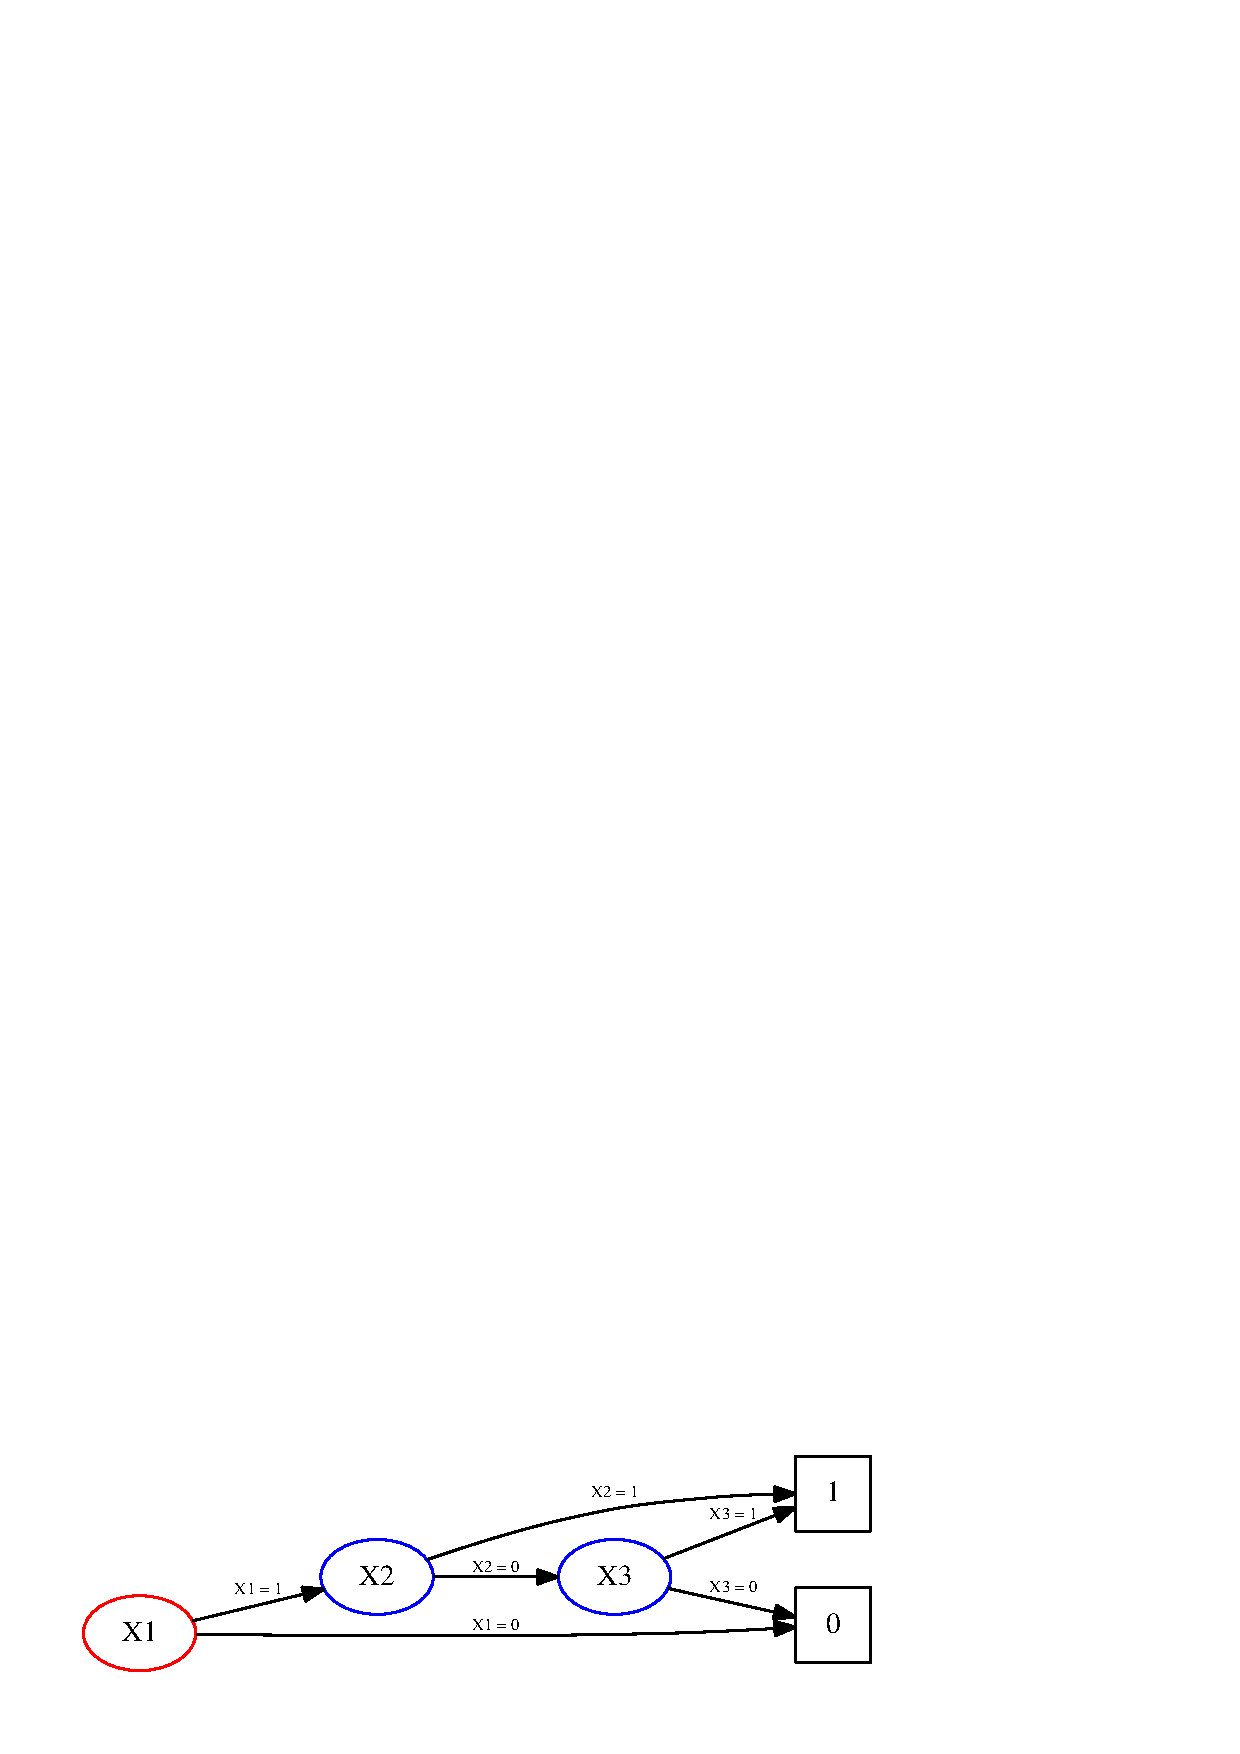
\includegraphics[height=3 cm]{./images/1a-LR.png}

\item $x_{1} \text{ xor } x_{2}$

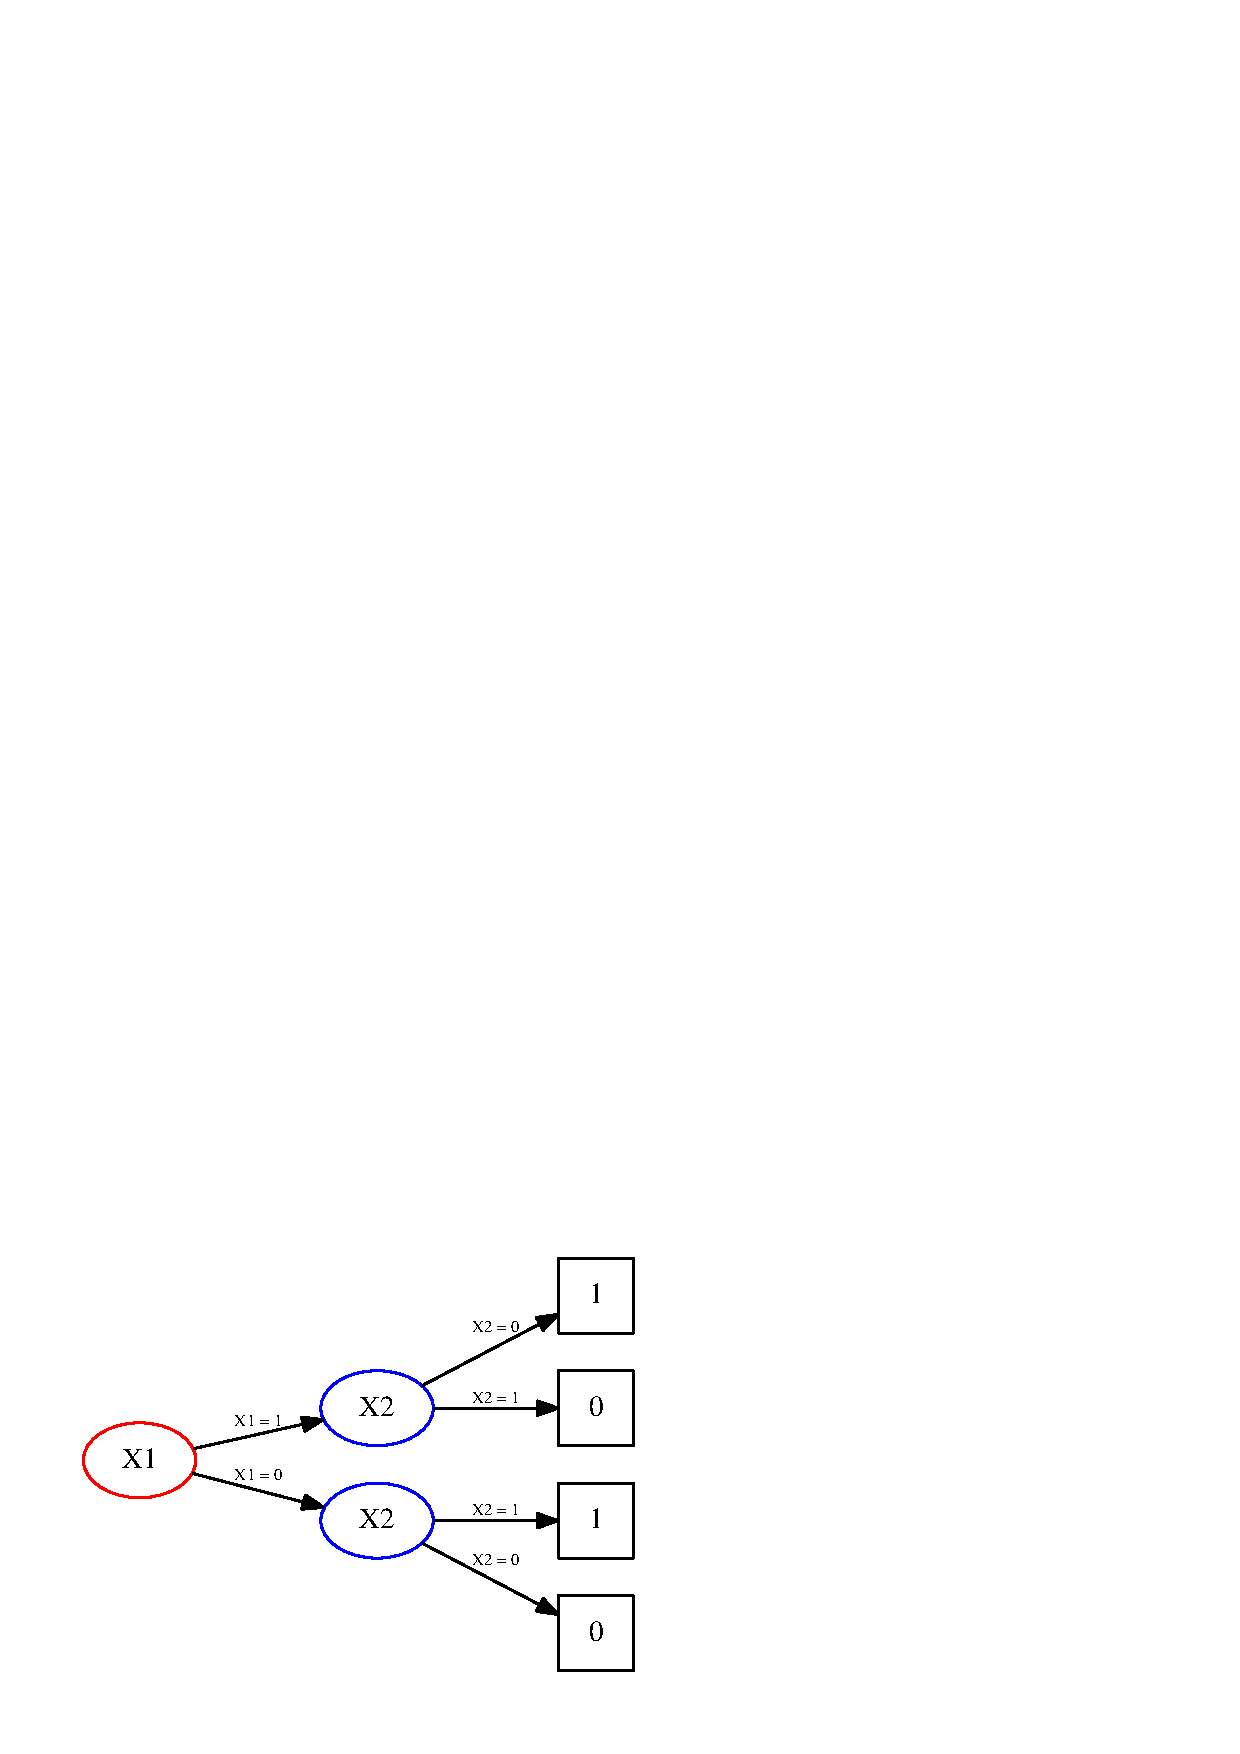
\includegraphics[height=5 cm]{./images/1b-LR.png}

\item The 2-of-3 function, whose value is true if at least two out of three Boolean features $x_{1}$, $x_{2}$, $x_{3}$ are true. After you represent this function using a decision tree, say whether you think using a decision tree to represent m-of-n functions is a good idea.

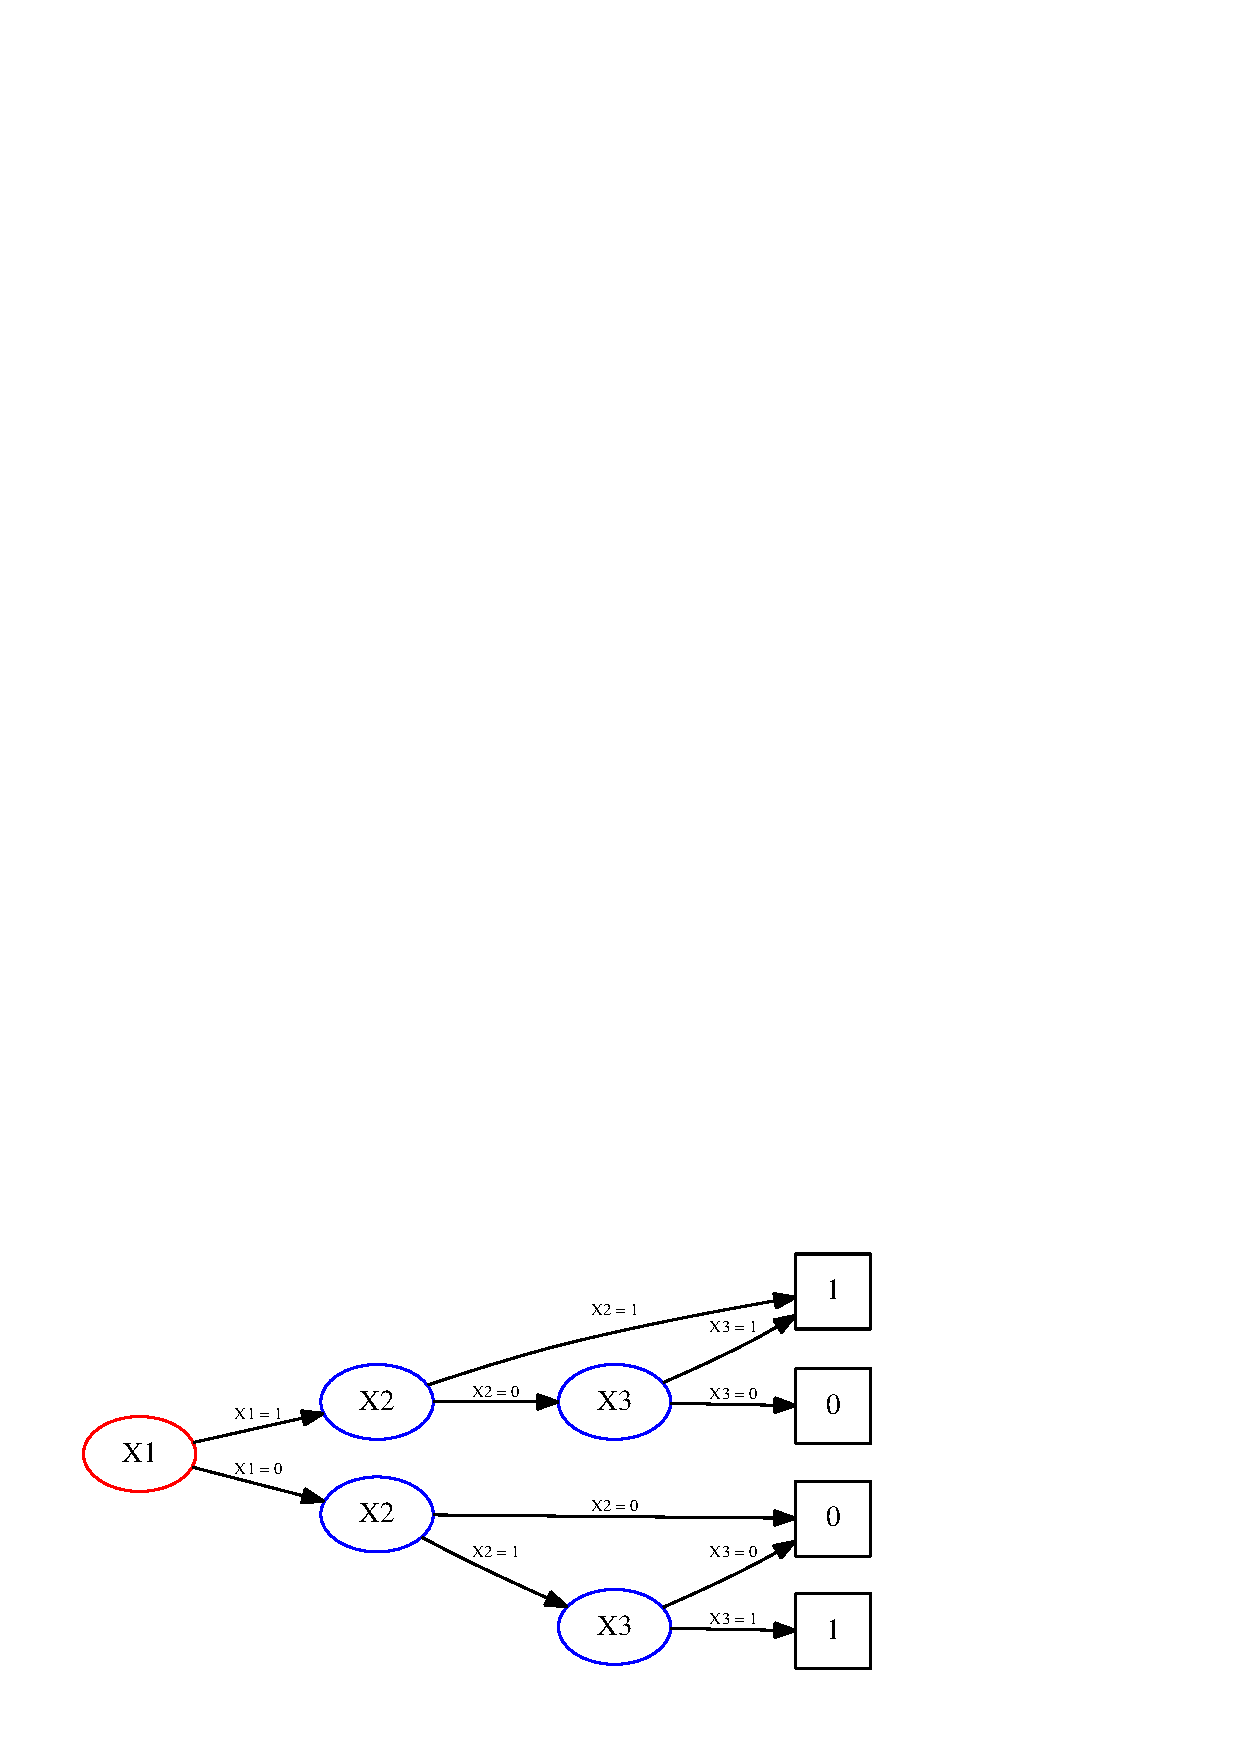
\includegraphics[height=5 cm]{./images/1c-LR.png}

Not a good idea for large data sets because you need $m\times n$ leaves for m-of-n functions. The maximum depth of the tree is of size $n$, however if $m=n$ then this is a good idea as it would have to check all of the values anyways and thus only needs to store $n+1$ leaves.
\end{itemize}

\item In this problem we will manually build a decision tree to decide whether to wait for a table at a restaurant.  Training data is given in Table 1.  There are four features: Friday (Yes or No), Hungry (Yes or No), Patrons (None, Some, Full), and Type (French, Italian, Thai, Chinese).
\begin{center}
\begin{tabular}{lllll}
\hline
Friday & Hungry & Patrons & Type & Wait?\\
\hline
No & Yes & Some & French & Yes\\
No & Yes & Full & Thai & No\\
No & No & Some & Chinese & Yes\\
Yes & Yes & Full & Thai & Yes\\
Yes & No & Full & French & No\\
No & Yes & Some & Italian & Yes\\
No & No & None & Chinese & No\\
No & Yes & Some & Thai & Yes\\
Yes & No & Full & Chinese & No\\
\hline
\end{tabular}
\end{center}
\begin{itemize}
\item How many possible functions are there to map these four features to a boolean decision? How many functions are consistent with the given training dataset?
\begin{itemize}
\item \textbf{Friday} has 2 possible values, so there are 2 combinations for it. \textbf{Hungry} also has 2 possible values, so 2 for it as well. \textbf{Patrons} has 3 combinations, and \textbf{Type} has 4 combinations. Therefore the total number of functions is $2\cdot 2\cdot 3\cdot 4 = 48$ different functions. If you want to include the decision for yes/no for every value, it would be double at 96.
\item Out of the 48 functions, in the training data 5 are labeled as a yes while there are only 9 needed to represent the data in the training data set.
\end{itemize}

\item What  is  the  entropy  of  the  labels  in  this  data? When calculating entropy, the base of the logarithm should be base 2.
\begin{align}
  \intertext{The entropy of a set of examples $S$ with binary classification is defined as}
  Entropy(S) &= H(S) = -p_{+}\log_{2}(p_{+}) -p_{-}\log_{2}(p_{-})\\
  p_{+} &= \text{Proportion of positive examples}\nonumber\\
  p_{-} &= \text{Proportion of negative examples}\nonumber\\
  \intertext{And this can be generalized in the following way:}
  H\left(\left\{ p_{1},p_{2},...,p_{k}\right\}\right) &= -\sum_{i=1}^{k}p_{i}\log\left( p_{i}\right)\\
  \intertext{We can caluclate the entropy of the entire data set with this equation, with the result being as follows:}\
  H(Y) &= -\left(\frac{5}{9}\right)\log_{2}\left(\frac{5}{9}\right) - \left(\frac{4}{9}\right)\log_{2}\left(\frac{4}{9}\right) \approx 0.99108
  \intertext{The entropy of each of the attributes is slightly different. One of them is calculated below while the others are tabulated in Table 2 but were calculated the same way.}
  \intertext{\underline{Hungry}}
  H_{H}(Yes) &= -\left(\frac{4}{5}\right)\log_{2}\left(\frac{4}{5}\right) - \left(\frac{1}{5}\right)\log_{2}\left(\frac{1}{5}\right) \approx 0.72193\\
  H_{H}(No)  &= -\left(\frac{1}{4}\right)\log_{2}\left(\frac{1}{4}\right) - \left(\frac{3}{4}\right)\log_{2}\left(\frac{3}{4}\right) \approx 0.20282\\
  H(Hungry) &= \left(\frac{4}{5}\right)H_{H}(Yes) + \left(\frac{1}{4}\right)H_{H}(No) \approx 0.78036
\end{align}
\begin{center}
\begin{tabular}{lr}
\hline
Attribute & Entropy\\
\hline
Friday & 0.91830\\
Hungry & 0.78036\\
Patrons & 0.14439\\
Type & 0.43609\\
\hline
\end{tabular}
\end{center}

\item What is the information gain of each of the features?

The information gain of the features is defined as
\begin{align}
Gain(S,A) &= Entropy(S) - \sum_{\nu \in Values(A)}\frac{|S_{\nu}|}{|S|}Entropy(S_{\nu})
\intertext{with $S_{\nu}$ being defined as the subset of examples where the value of attribute $A$ is set to the value of $\nu$. The entropy of the entire set of data $(H(Y))$ was calculated back in Equation (3). Using this value, and the value from Equation (6), an example calculation of the {\em Information Gain} for the attribute {\bf Hungry} can be calculated. The others are similar and instead of being calculated one by one are tabulated as the method is the same.}
Gain(Y,Hungry) &\approx 0.99108 - 0.78036 \approx 0.21072
\end{align}
\begin{center}
\begin{tabular}{lr}
\hline
Attribute & Information Gain\\
\hline
Friday & 0.07305\\
Hungry & 0.21072\\
Patrons & 0.84669\\
Type & 0.55409\\
\hline
\end{tabular}
\end{center}

\item Which attribute will you use to construct the root of the tree using the ID3 algorithm?
\begin{itemize}
\item The ID3 Algorithm chooses the root based on the largest amount of information gain, so it would be \emph{Patrons}. It then goes down the list and chooses the next ones as the next highest information gain and so on until the tree describes the data.
\end{itemize}
\item Using the root that you selected in the previous question, construct a decision tree that represents the data. You do not have to use the ID3 algorithms here, you can show any tree with the chosen root.

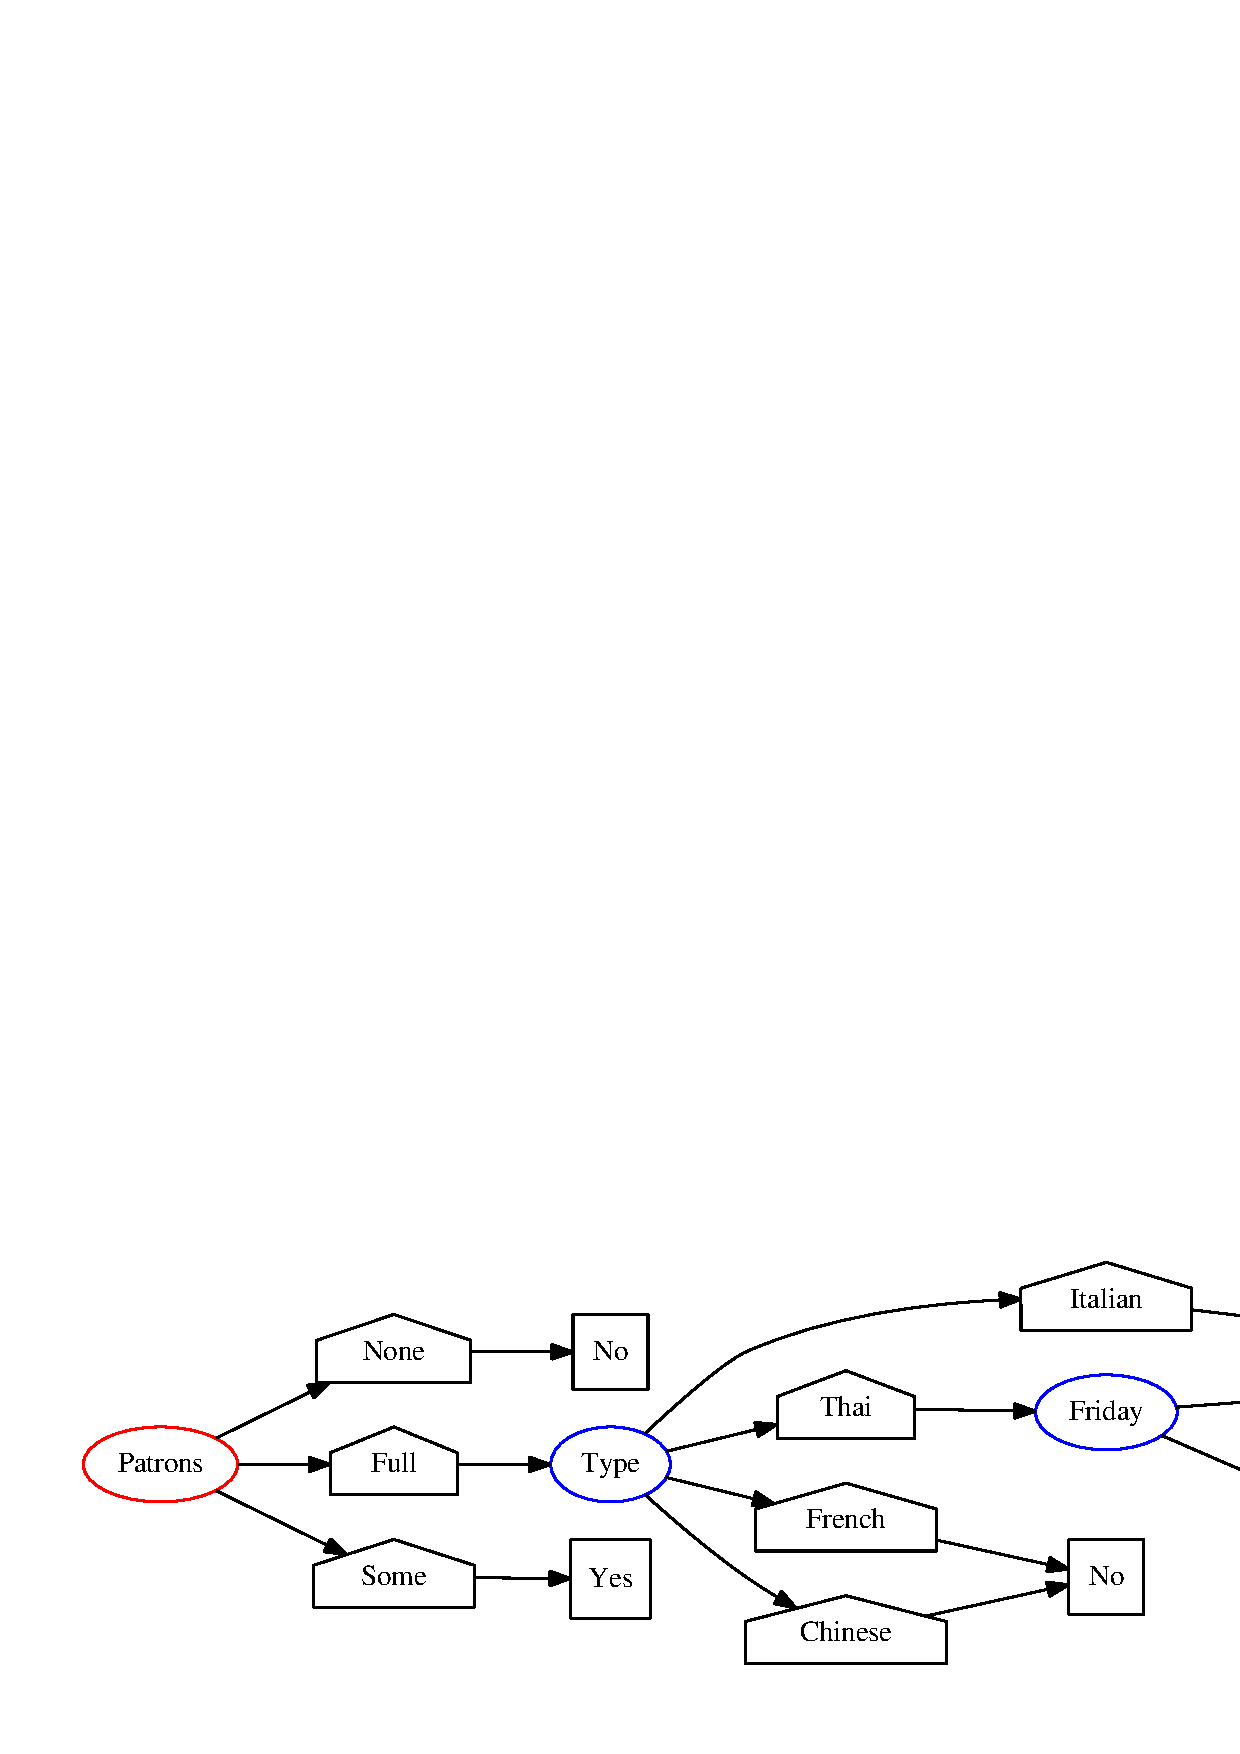
\includegraphics[width=.9\linewidth]{./images/2e.png}

\item Suppose you are given three more examples, listed in table 2. Use your decision tree to predict the label for each example. Also report the accuracy of the classifier that you have learned.
\begin{center}
\begin{tabular}{lllll}
\hline
Friday & Hungry & Patrons & Type & Wait?\\
\hline
Yes & Yes & Full & Italian & No\\
No & No & None & Thai & No\\
Yes & Yes & Full & Chinese & Yes\\
\hline
\end{tabular}
\end{center}

\begin{itemize}
\item Using these examples with the decision tree, only 1 of the test cases is valid, the middle one, while the first and last case fail. In the decision tree, from the learning data, \emph{Italian} is technically not needed for coming to the conclusions, but it was included into it as it failed during the test data. However, even though Italian was added, the solution was only taken from the learning data and not the test data. This was more to just stop it from "breaking" in not finding \emph{Italian} in the type.
\end{itemize}
\end{itemize}

\item Recall that the ID3 algorithm identies the best attribute to create the decision tree using the information gain heuristic. This heuristic uses the difference between the entropy of the data and the expected entropy of the splits to identify the root attribute. Here, we use entropy as a way quantify \emph{impurity} of labels in the data.  However, we could use other measures of impurity instead of entropy within the same definition. In this question, we will explore the use of other impurity measures. 
\begin{itemize}
\item One natural way to define impurity is to measure the misclassification rate.  This measures the error that we would have made if we had chosen the most frequent label. It is defined as
\begin{equation}
    Misclassification(S) = 1 - \max_{i}p_{i}
  \end{equation}
Here, $p_{i}$ is the fraction of examples that have a label $i$ and the maximization is over all labels.
\begin{itemize}
\item Write down the definition of the information gain heuristic that uses the misclassification rate as its measure of impurity instead of entropy.
\begin{align}
\intertext{The definition of $Information\ Gain$ for a given attribute $A\in S$ is}
H(A) &= Entropy(S) \sum_{\nu\in Values} \frac{\left| S_{\nu}\right|}{\left| S\right|}Entropy\left( S_{\nu}\right)
\intertext{By applying the above equation of $Misclassification$ to this formula, we get the information gain heuristic that uses $Misclassification$ instead of $Entropy$}
&\left[ 1-\max_{i} \left(p_{i}\right)\right] - \sum_{\nu\in Values}\frac{\left| S_{\nu}\right|}{\left| S\right|} \left[ 1 - \max_{\nu}\left( p_{\nu}\right)\right] 
\end{align}
\item Use your new heuristic to identifiy the root attribute for the data in Table 1.
\begin{itemize}
\item Using the above equation for information gain, the misclassification values were calculated. Below, I show one example about how one of them was calculated, while the other values are tablulated in the table below.

\ \\
\intertext{\underline{Type}}\\
\intertext{M(S_{Hungry}) = \underbrace{\left((1-\frac{5}{9}\right))}_{M(S)} - \underbrace{\frac{5}{9}\left( 1- \frac{4}{9}\right)}_{Hungry} = \frac{1}{3}\\
\intertext{$In the above calucation, the part of the equation labeled with $M(S)$ is the total Misclassification rate over the labels, while the section labeled with "Hungry" is the misclassification rate for the Attribute Hungry. To calculate this, the most common value (irrespective of the label) was $yes$ with a probability of $\frac{5}{9}$, and the probability that it was labeled $yes$ was $\frac{4}{9}$, which is where the numbers came from. If you used the above equation for the misclassification rate, you get $\frac{1}{3}$ for the misclassification rate for $Hungry.$}
\begin{center}
\begin{tabular}{lr}
\hline
Attribute & Information Gain\\
\hline
Friday & 0.22222\\
Hungry & 0.33333\\
Patrons & 0.22222\\
Type & 0.22222\\
\hline
\end{tabular}
\end{center}

From the above table, it's easy to see that if we want to pick the root with the highest information gain that it would be \emph{Hungry}.
\end{itemize}
\end{itemize}

\item Another heuristic that is used to define impurity is the Gini coefficient, which is defined as
\begin{equation}
    Gini(S) = \sum_{i}p_{i}(1-p_{i})
  \end{equation}
Use the Gini coefficient to identify the root attribute for the training data in Table 1.
\begin{align}
\intertext{Using the above equation, we can calculate the Gini Coefficient for the entire data as follows. We need to do this before using it to calculate the information gain of each attribute.}
G(S) &= \sum_{i}p_{i}\left( 1-p_{i}\right) = \underbrace{\frac{5}{9}\left( 1-\frac{5}{9}\right)}_{yes} + \underbrace{\frac{4}{9}\left( 1-\frac{4}{9}\right)}_{No} = \frac{40}{81} \approx 0.49383\\
\intertext{This is the base for the overall set of data. Below, one example calculation is made and described, while the information gain for all of the attributes is tabulated below.}
G\left( S_{Friday}\right) &= \underbrace{\frac{6}{9}\left[ \underbrace{\frac{2}{6}\left( 1-\frac{2}{6}\right)}_{Label: No} + \underbrace{\frac{4}{6}\left( 1 - \frac{4}{6}\right)}_{Label: Yes}\right]}_{Value: No} + \underbrace{\frac{3}{9}\left[ \underbrace{\frac{1}{3}\left( 1-\frac{1}{3}\right)}_{Label: Yes} + \underbrace{\frac{2}{3}\left( 1 - \frac{2}{3}\right)}_{Label: No}\right]}_{Value: Yes} = \frac{31}{90} \approx 0.3\bar{4}\\
\intertext{In the above calculation, the first set of data looks at the probability for the data that had a $Value$ of "No," and looks at the corresponding probabiltiies of the labels. In the attribute $Friday$, there are 6 values of No, and 3 of Yes. In the first set, only $\frac{2}{6}$ of those values map to a No Label, while the remaining $\frac{4}{6}$ map to a Yes label. In the $Value:\ Yes$ category, there are only $\frac{3}{9}$ that have values of Yes in Friday, and of those, only $\frac{1}{3}$ map to a yes label while the remaining $\frac{2}{3}$ map to a no label.}\nonumber
\end{align}
\begin{center}
\begin{tabular}{lrr}
\hline
Attribute & Gini Coefficient & Information Gain\\
\hline
Friday & 0.44444 & 0.04939\\
Hungry & 0.34444 & 0.14939\\
Patrons & 0.16666 & 0.32717\\
Type & 0.40741 & 0.08642\\
\hline
\end{tabular}
\end{center}
The attribute with the largest Gini coefficient is \emph{Patrons}, which is what the root would be if using the Gini Coefficient to build the tree.
\end{itemize}
\end{enumerate}
\section{Nearest Neighbors}
\label{sec-2}

The nearest neighbors algorithm partitions the space of examples into regions corresponding to  different  labels.   In  two  dimensions,  the  decision  boundaries  can  be  represented  as  a Voronoi diagram, which shows regions of the plane associated with each label.
\begin{enumerate}
\item Using the Euclidean distance measure between points, show a Voronoi map corresponding to the nearest neighbor classifiation of the following four points.  (That is, draw a diagram that shows how the nearest neighbor classification of the following four points partitions the two dimensional plane.)

\begin{center}
\begin{tabular}{lrr}
\hline
Label & x & y\\
\hline
A & 1 & 1\\
A & 1 & -1\\
B & -1 & -1\\
C & 2 & -2\\
\hline
\end{tabular}
\end{center}

\begin{itemize}
\item For this part of the assignment, I wrote a program that calculated and plotted the given Voronoi Diagram for different metrics. I followed the defintiion of the distances and Dr. Vivek Srikumar stated that I didn't have to include the code for this section.  The figure for using the Euclidean distance can be seen below.

\includegraphics[height=8 cm \centering]{./images/NN_3a.png}
\end{itemize}
\end{enumerate}


\begin{enumerate}
\item Using the city-block distance measure, show a Voronoi map corresponding to the nearest neighbor classification of the following three points.

(Recall that the city-block measure/Manhattan distance/$L_{1}$ distance/taxicab metric between two points ${\mathbf x}$, ${\mathbf y}$ in the $n$-dimensional space $\mathbb{R}^{n}$ is defined as $\sum_{i=1}^{n}\left| x_{i}-y_{i}\right|$.)

\begin{center}
\begin{tabular}{lrr}
\hline
Label & x & y\\
\hline
A & 1 & 1\\
B & -1 & -1\\
C & 2 & -2\\
\hline
\end{tabular}
\end{center}

\includegraphics[height=8 cm \centering]{./images/NN_3b.png}
\end{enumerate}


\begin{enumerate}
\item Can you design a \emph{tiny} training data set such that nearest-neighbor classification using Euclidean distance and Manhattan distance will give you different results? To answer this question, you can assume the data are in two-dimensional plane. Each data point is specified using its Cartesian coordinate, just like in previous part of this problem.  Show your training set and one test example so that the two distances will give your conflicting results on that test example.

\begin{center}
\begin{tabular}{lrr}
\hline
Label & x & y\\
\hline
A & 1.5 & 1.5\\
B & -1.5 & -1.0\\
B & 1.0 & -2.0\\
C & -0.5 & 1.0\\
\hline
\end{tabular}
\end{center}
\end{enumerate}


\includegraphics[height=8 cm \centering]{./images/NN_3c1.png}

\includegraphics[height=8 cm \centering]{./images/NN_3c2.png}

\section{Experiment}
\label{sec-3}

In  this  question,  you  will  implement  decision  tree  learners  and  the  $K$-nearest  neighbors algorithms.   Also  you  will  learn  to  select  the  proper $K$ value  in  your $K$-nearest  neighbor algorithm using a technique called \emph{cross-validation}.

This problem uses the Tic-Tac-Toe Endgame Data set from the UCI machine learning repository.   Each  data  point  has  9  features  indicating  the  9  locations  on  the  Tic-Tac-Toe game board.  The feature can have one of the three values:  x, o, and b (for blank).  The label is positive or negative, indicating whether player x wins or not. Your goal is to use various learning algorithms on the training data to train a predictor and see how well it does on the test data. You may use any programming language for your implementation.  However, the graders should be able to execute your code on the CADE machines.

Your goal is to use various learning algorithms on the training data to train a predictor and see how well it does on the test data.

You may use any programming language for your implementation. However, the graders should be able to execute your code on the CADE machines.

\subsection{Cross Validdddddation}
\label{sec-3-1}

The value $K$ is a hyper-parameter to the $K$ nearest neighbor algorithm.  You will see later in the semester that many machine learning algorithm (SVM, logistic-regression etc) have some hyper-parameters as their input.  One way to determine a proper value for the hyper-parameter is to use a technique called cross-validation.

As usual we have a training set and a test set.  Some of the training data is put aside, and when training is finished,  the resulting classifier is tested on the held out data.  This allows you get get an idea of how well the particular choice of hyper-parameters does.  Since you did not train on your whole dataset you may have introduced a bias.  To correct for this, you will need to train many classifiers with different subsets of the training data removed.

For problems with small data sets, a popular method is the leave-one-out approach.  For each example, a classifier is trained on the rest of the data and the chosen example is then evaluated.   The  performance of  the  classifier  is  the  average  accuracy  on  all  the  examples. The downside to this method is for a data set with $n$ examples you must train $n$ different classifiers.  Of course, this is not practical for the data set you will use in this problem, so you will hold out subsets of the data many times instead.

Specifically, for this problem, you should implement $k$-fold cross validation to identify the hyperparameter $K$ (Don't confuse $k$ with $K$, they are different). The general approach for $k$-fold cross validation is the following: Suppose you want to evaluate how good a particular hyper-parameter is. You split the training data into $k$ parts. Now, you will train your model on $k-1$ parts with the chosen hyper-parameter and evaluate the trained model on the remaining part. You should repeat this $k$ times, choosing a different part for evaluation each time. This will give you $k$ values of accuracy. Their \emph{average cross-validation accuracy} gives you an idea of how good this choice of the hyper-parameter is. To find the best value of the hyper-parameter, you will need to repeat this procedure for different choices of the hyper-parameter. Once you find the best value of the hyper-parameter, use the value to retrain your classifier using the entire training set.
\subsection{Data Files}
\label{sec-3-2}

You can find the data on the assignments page of the class website in a file called \texttt{tic-tac-toe.zip}. It consists of six training files (used for 6-fold cross validation in KNN), and one test file, which you will use for training and testing respectively.

\begin{enumerate}
\item Implement a decisddddddddddion tree data structure. (Remember that the decision tree need not be a binary tree!)
\item Implement the ID3 learning algorithm for your decision tree implementation. For debugging your implementation, you can use the previous toy examples from the homework like the restaurant data from Table 1. Report the accuracy of your decision tree on the test data. \emph{Important:} You need to combine all training examples in all six training files when you train your decision tree. Don't just train your tree using only one training file.
\item Implement a $K$ Nearest Neighbor classifier for a general $K$. Note that your features are only categorical. So you have to make choices about how to measure distances between them. For example, you could consider using the Hamming distance between the feature representations.
\item Implement cross-validation. Run 6-fold cross-validation $(k=6)$ to select the best $K$ value from $K\in \{1,2,3,4,5\}$. The training data are already separated into six folds for you, each fold is a separate file. Report the average cross-validation accuracy for each choice of $K$. Use the best value of $K$ to retrain your classifier on the entire train data set. Report its accuracy on the test data.
\end{enumerate}
\subsection{What to hand in for this problem}
\label{sec-3-3}
\begin{enumerate}
\item The report should detail your experiments. For each step, explain in no more than a paragraph or so how your implementation works. You may provide the results for the final step as a table or graph.
\item \emph{Your code should run on the CADE machines.} You should include a shell script, \texttt{run.sh}, that will execute your code in the CADE environment. Your code should produce similar output to what you include in your report. 
You are responsible for ensuring that the grader can execute the code using only the included script. If you are using an esoteric programming language, you should make sure that its runtime is available on CADE.
\item The points for this question will be as follows: 20 points for the decision tree part, 20 points for the $K$-NN part and 15 points for your report.
\item Please do not hand in binary files! We will not grade binary submissions.
\end{enumerate}
\subsection{ID3}
\label{sec-3-4}
In implementing the ID3 Decision tree algorithm, the background of it is to go through each column and calculate the information gain for each of the values and then for the labels as well. Equation 1 and Equation 2 were used to calculate the information gain. After the informaetion gain of each attribute was choosen, this was used as the "root" for the level the tree was at. 

When buidling the tree, it fills every available spot with a "Default Value" for just in case a value is not found in the list when doing a test/classification. It looks for the most common label at the level that is being evaluated and sets it to that default level for all positions. Then, when filling the tree, any values that actually exist overwrite the default value, and any value that doesn't, keeps the default value.

The ID3 Alogirhtm minimizes the tree height based off of the information gain, where the next attribute to be decided on is the one with the highest information gain/lowest entropy. After building the tree, the program reads in the test data, where it then traverses the tree for each test data to try and classify it. After doing so, if it finds a case that matches in the tree, it returns \verb~psotive~ or \verb~negative~ for the label of the data. If the data was not found in the tree, then it gives it a "best guess" for the data and will return the default value at that level if it ran into a dead end.

\verb~*************************************************~

\verb~Running ID3 over the data~

\verb~*************************************************~

\verb~Out of the test set, 175/196 were correct, while 21/196 were wrong~
\subsection{K Nearest Neighbors}
\label{sec-3-5}
For K Nearest Neighbors (K-NN), each row of the data for any data that was trained on was read into a single array. The actual vaues \verb~x~, \verb~o~, \verb~b~, \verb~postive~ and \verb~negative~ were stored in the array instead of turning it into numerical representations.

When the test set was used, the Hamming Distance was used on the array to try and classify the data. The folloowing example shows how this works.

\verb~['o', 'x', 'x', 'x', 'x', 'o', 'o', 'o', 'x', 'negative']~

\verb~['x', 'x', 'x', 'o', 'o', 'b', 'b', 'b', 'b', 'negative']~

In this above example, each index of each "game" is compared, except for the results. All but the second and third columns are wrong, which produces a Hamming Distance of 7 then. So the Hamming Distance for each of the test cases was computed for all of the training data, and the closest $K$ are stored. In the method implemented, the smallest distance was calculated between the test game and all the other games, which we can call $\epsilon$. Then, after calculating $\epsilon$, the test data is compared against the training data again, and it reads the labels of the first $K$ $\epsilon$ in the training data, and if $K$ $\epsilon$ didn't exist, then it incremented $\epsilon$ by 1, and those are compared until the $K$ closest neighbors are achieved.

While there would be better implementations of this, for example reading in all $\epsilon$ neighbors and then calculating the $K$ relative smallest, this was a highly effective method that was accurate to over 90\% in the best case.

In $k$-fold cross validation, to obtain the best $K$, $K$ was tested over the range \{1,2,3,4,5\} to find the best $K$ to use with the data. To do this, an example of this iteration will be shown. First, set $K=1$ and train over the files 2-6 and test on the first file. Store the accuracy of this run, and continue with $K=1$ but train on files \{1,3,4,5,6\} and test on the second one. This was iterated over all of the files and after testing on all the files (by leaving one out) abnd taking the average of the accuracy for each value of $K$, $K$ was incremented and the processess was repeated until $K$ reached 5. After testing each value of $K$, the $K$ with the best accuracy was choosen, and the data was retrained over ALL of the training data and then applied to the one test data that we had and looked at the accuracy. This would optimize the learning parameter used over the test data without showing the test data to the program until the end, and optimizing the learning algorithm.

\verb~*************************************************~

\verb~Running K-nearest neighbors over the data~

\verb~*************************************************~

\verb~---------------------------------------------~

\verb~For K = 1 the average accuracy is 0.803: 102/127~

\verb~---------------------------------------------~

\verb~For K = 2 the average accuracy is 0.803: 102/127~

\verb~---------------------------------------------~

\verb~For K = 3 the average accuracy is 0.858: 109/127~

\verb~---------------------------------------------~

\verb~For K = 4 the average accuracy is 0.858: 109/127~

\verb~---------------------------------------------~

\verb~For K = 5 the average accuracy is 0.921: 117/127~

\verb~---------------------------------------------~

\verb~The max K from k-fold cross validation is K = 5.~

\verb~Setting it and retesting over the entire dataset~

\verb~---------------------------------------------~

\verb~For k = 5 nearest neighbors, 187/196 are correct using the whole training set~
% Emacs 24.5 (Org mode 8.2.10)
\end{document}
